% ==========================================
% BAB V RENCANA SELANJUTNYA
% ==========================================
\chapter{RENCANA SELANJUTNYA}
\label{chap:rencana-selanjutnya}

Bab ini merinci langkah-langkah implementasi teknis, jadwal pelaksanaan, dan strategi pengujian yang akan dilakukan untuk memvalidasi efektivitas desain solusi yang telah dirancang, serta analisis risiko yang mungkin dihadapi.

\section{Rencana Implementasi}
\label{sec:rencana_implementasi}
Implementasi purwarupa akan dibangun sebagai aplikasi berbasis web (\textit{web-based}) untuk menjamin aksesibilitas tanpa instalasi khusus di sisi pengguna. Strategi implementasi dirancang untuk memaksimalkan penggunaan layanan \textit{cloud} tingkat gratis (\textit{free tier}) guna menekan biaya operasional, dengan pemilihan teknologi yang didasarkan pada kebutuhan spesifik sistem adaptif.

\subsection{Spesifikasi Lingkungan Pengembangan}
Pengembangan dilakukan secara lokal menggunakan perangkat komputasi standar dengan spesifikasi minimum prosesor setara Intel Core i5/AMD Ryzen 5 dan memori 8 GB untuk menjalankan kontainerisasi layanan. Perangkat lunak pendukung meliputi Visual Studio Code sebagai editor kode, Git untuk manajemen versi, dan Postman untuk pengujian API.

Arsitektur sistem akan diimplementasikan menggunakan kumpulan teknologi (\textit{tech stack}) berikut:

\begin{enumerate}
    \item \textit{Backend} - Python (FastAPI):
    bahasa pemrograman yang dipilih adalah Python karena dukungan ekosistem pustaka komputasi ilmiah (seperti NumPy) yang matang, yang sangat krusial untuk menangani perhitungan matematis algoritma \textit{Elo rating} dan logika statistik \textit{Re-ranking} secara presisi dan efisien. Kerangka kerja FastAPI dipilih untuk memastikan performa tinggi dalam melayani permintaan data secara asinkron.
    
    \item \textit{Frontend} - React.js:
    pengembangan antarmuka menggunakan React.js karena arsitektur berbasis komponen dan mekanisme \textit{Virtual DOM}-nya memungkinkan pembaruan tampilan yang sangat responsif. Hal ini penting untuk menyajikan grafik kompetensi \textit{real-time} dan interaksi formulir rubrik yang dinamis tanpa membebani peramban pengguna.
    
    \item \textit{Database} - PostgreSQL:
    mengingat sifat data skor Elo yang transaksional dan bergantung pada integritas riwayat sebelumnya (\textit{stateful}), sistem menggunakan PostgreSQL. Basis data ini menawarkan kepatuhan ACID yang ketat serta fitur MVCC (\textit{Multi-Version Concurrency Control}) yang andal untuk menangani konkurensi data saat banyak siswa melakukan pengumpulan tugas secara bersamaan.
\end{enumerate}

Sistem akan di-\textit{deploy} menggunakan layanan \textit{cloud} terkelola (\textit{managed services}) yang menyediakan kuota gratis, yaitu Supabase untuk basis data, Render/Railway untuk layanan \textit{backend}, dan Vercel untuk \textit{hosting frontend} dan jaringan pengiriman konten (CDN).

\subsection{Persiapan Materi dan Instrumen (\textit{Cold-Start})}
Agar sistem dapat berfungsi optimal pada fase awal saat data historis belum tersedia, diperlukan persiapan instrumen sebagai berikut:

\begin{enumerate}
    \item \textbf{Penyusunan Bank Soal:} Akan disusun minimal 20 butir latihan
    soal dengan topik Pemodelan dan Manajemen Basis Data. Jumlah ini ditetapkan
    sebagai ambang batas minimum data poin yang diperlukan algoritma Elo untuk
    mencapai konvergensi estimasi kemampuan awal ($R_0$) ke kemampuan sebenarnya
    ($\theta$). Kalibrasi tingkat kesulitan awal ($D_j$) akan dilakukan secara
    manual oleh Asisten Laboratorium Basis Data. Pemilihan topik latihan
    disesuaikan dengan latar belakang partisipan dan ketersediaan sumber daya.
    
    \item \textbf{Penyusunan Rubrik Penilaian:} Instrumen penilaian sejawat
    disusun mengacu pada revisi Taksonomi Bloom (khususnya aspek Analisis dan
    Evaluasi) untuk menjamin objektivitas penilaian tugas. Selain itu, disiapkan
    pula Rubrik Kualitas Umpan Balik yang diadopsi dari penelitian terdahulu
    untuk keperluan validasi kualitas komentar siswa oleh LLM.
\end{enumerate}

\section{Rencana Jadwal Pelaksanaan}
\label{sec:timeline}
Penelitian dan pengembangan sistem direncanakan berlangsung selama 4 bulan, terhitung mulai Januari 2026 hingga April 2026. Alokasi waktu disusun dengan memberikan porsi terbesar pada fase pengembangan teknis untuk memastikan kehandalan logika adaptif sebelum pengujian dilakukan.
Pada Gambar \ref{fig:gantt_chart} diperlihatkan linimasa kegiatan utama penelitian yang direncanakan.

\begin{figure}[!ht]
    \centering
    % Placeholder untuk gambar Gantt Chart
    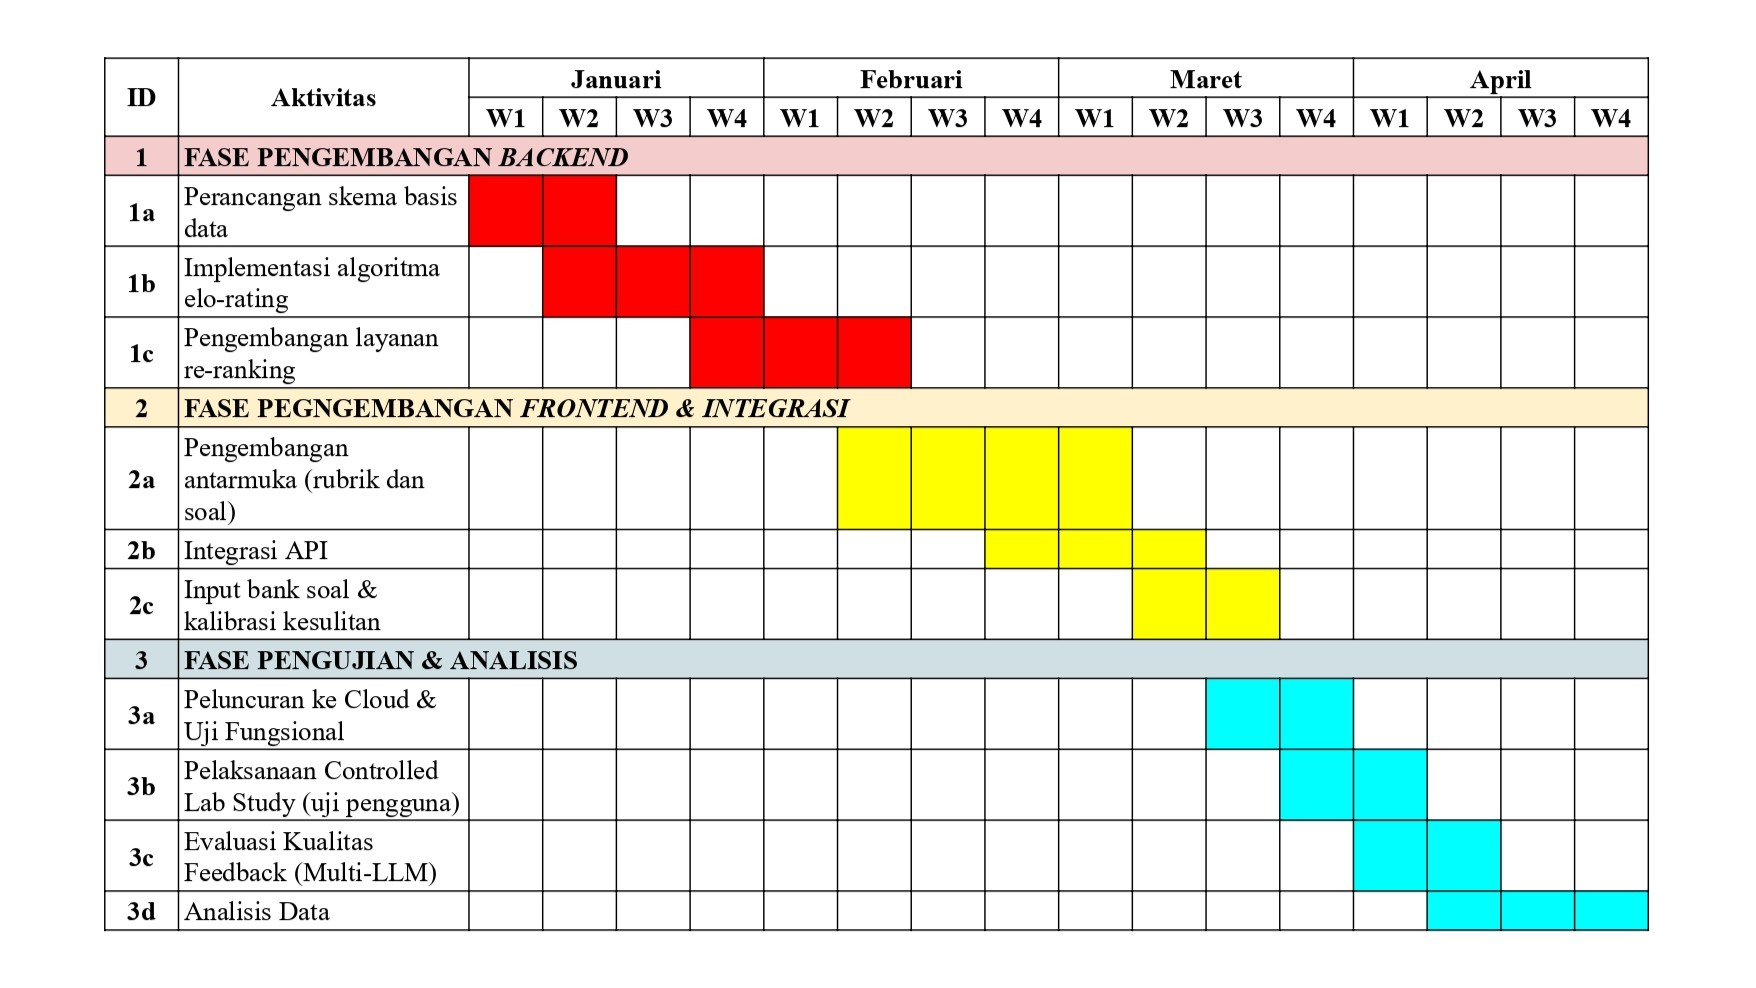
\includegraphics[width=0.95\textwidth]{image/gantt_chart_plan.jpg}
    \caption{Gantt Chart Rencana Jadwal Pelaksanaan (Januari - April 2026)}
    \label{fig:gantt_chart}
\end{figure}

Rincian fokus kegiatan per bulan dijelaskan sebagai berikut:

\begin{enumerate}
    \item \textbf{Bulan 1 (Januari 2026):}
    kegiatan difokuskan sepenuhnya pada pengembangan sisi \textit{backend}. Minggu-minggu awal dialokasikan untuk perancangan skema basis data PostgreSQL yang matang, diikuti dengan implementasi algoritma \textit{Elo rating}. Pengembangan logika layanan \textit{Re-ranking} dimulai pada akhir bulan ini.
    
    \item \textbf{Bulan 2 (Februari 2026):}
    awal bulan digunakan untuk merampungkan layanan \textit{Re-ranking}. Fokus kemudian beralih ke pengembangan antarmuka pengguna (\textit{Front-end}) menggunakan React.js, khususnya pada komponen interaktif seperti formulir rubrik penilaian dan visualisasi grafik kompetensi.
    
    \item \textbf{Bulan 3 (Maret 2026):}
    kegiatan utama meliputi integrasi penuh antara API \textit{backend} dan \textit{frontend}, serta input konten bank soal (20 butir) yang telah dikalibrasi. Pada paruh kedua bulan Maret, sistem akan di-\textit{deploy} ke infrastruktur \textit{cloud} untuk menjalani uji fungsional internal (\textit{alpha testing}) demi memastikan kesiapan sebelum melakukan pengujian yang melibatkan partisipan eksternal.
    
    \item \textbf{Bulan 4 (April 2026):}
    pelaksanaan \textit{Controlled Lab Study} dengan partisipan (sesi \textit{micro-learning}) dijadwalkan pada awal bulan. Sisa waktu dialokasikan untuk evaluasi intensif, meliputi validasi kualitas \textit{feedback} menggunakan \textit{Multi-LLM Voting}, perhitungan \textit{Normalized Learning Gain} (NLG), dan analisis log sistem.
\end{enumerate}

\section{Rencana Anggaran Biaya (RAB)}
\label{sec:rab}
Berdasarkan strategi pemilihan teknologi \textit{open-source} dan layanan \textit{cloud free-tier}, proyek ini dirancang untuk dilaksanakan dengan biaya kapital nol rupiah (Rp 0). Rincian estimasi biaya disajikan pada Tabel \ref{tbl:rab}.

\begin{table}[H]
    \centering
    \caption{Rencana Anggaran Biaya}
    \label{tbl:rab}
    \begin{tabular}{|p{0.05\textwidth}|p{0.35\textwidth}|p{0.30\textwidth}|p{0.20\textwidth}|}
        \hline
        \textbf{No} & \textbf{Komponen} & \textbf{Spesifikasi/Layanan} & \textbf{Biaya (Rp)} \\
        \hline
        1 & \textit{Hosting Frontend} & Vercel (\textit{Hobby Tier}) & 0 \\
        \hline
        2 & \textit{Hosting Backend} & Render/Railway (\textit{Free}) & 0 \\
        \hline
        3 & \textit{Cloud Database} & Supabase (\textit{Free Tier}) & 0 \\
        \hline
        4 & \textit{Domain} & Subdomain dari Provider & 0 \\
        \hline
        5 & Layanan LLM & Hugging Face Inference API / Google Gemini API (\textit{Free Tier}) & 0 \\
        \hline
        6 & Perangkat Pengembangan & Laptop Pribadi (Aset) & 0 \\
        \hline
        7 & Koneksi Internet & Kuota Pribadi (\textit{Sunk Cost}) & 0 \\
        \hline
        \multicolumn{3}{|r|}{\textbf{Total Estimasi Biaya}} & \textbf{Rp 0} \\
        \hline
    \end{tabular}
\end{table}

\section{Desain Pengujian dan Evaluasi}
\label{sec:desain_pengujian}
Untuk mengukur keberhasilan sistem dalam memitigasi isolasi
pembelajaran, pengujian dilakukan menggunakan metode
\textbf{\textit{Controlled Lab Study}} (Studi Laboratorium
Terkontrol) dengan desain \textit{One-Group Pretest-Posttest}.
Pendekatan sesi tunggal intensif ini dipilih untuk mengisolasi
variabel pengganggu (\textit{confounding variables}) seperti
pembelajaran eksternal di kelas, sehingga peningkatan kompetensi
dapat diatribusikan secara langsung pada interaksi sistem,
sekaligus meminimalkan gangguan terhadap jadwal akademik
partisipan (non-invasif).

\subsection{Prosedur Etika dan Privasi Data}
Sebelum pelaksanaan eksperimen, seluruh partisipan diwajibkan
untuk menyetujui \textit{Informed Consent} yang menyatakan
kesediaan mereka agar data aktivitas pembelajarannya digunakan
untuk kepentingan riset. Untuk menjamin privasi dan objektivitas
penilaian sesuai dengan NFR-05, sistem menerapkan mekanisme
\textbf{\textit{Double-Blind Peer Assessment}}. Dalam mekanisme
ini, identitas siswa yang dinilai (\textit{assessee}) disamarkan
dari penilai, begitu pula sebaliknya, sehingga penilaian
didasarkan murni pada kualitas pekerjaan tanpa dipengaruhi
bias relasional.

\subsection{Skenario Pengujian (\textit{Micro-learning Session})}
Partisipan yang dilibatkan berjumlah 10-15 orang mahasiswa tingkat sarjana. Sesi pengujian berlangsung selama 90-120 menit dengan alur sebagai berikut:

\begin{enumerate}
    \item \textbf{Fase \textit{Pre-test} (15 Menit):} 
    Partisipan mengerjakan tes awal untuk menetapkan \textit{baseline} pengetahuan dan inisialisasi skor Elo awal.
    
    \item \textbf{Fase Interaksi Sistem (45 Menit):} 
    Partisipan mengerjakan latihan adaptif SQL. Sistem dikonfigurasi untuk memicu fitur \textit{Peer Assessment} ketika mendeteksi pola stagnasi skor.
    
    \item \textbf{Fase Intervensi Sosial (30 Menit):} 
    Partisipan melakukan penilaian sejawat terhadap rekan yang dipilihkan oleh algoritma \textit{Re-ranking} (heterogen). Evaluasi hasil \textit{peer assessment} pada tahap ini dilakukan melalui dua mekanisme:
    \begin{enumerate}
        \item \textbf{\textit{Helpful Vote}:} Penerima masukan (\textit{assessee}) memberikan vote apakah masukan membantu (validasi subjektif).
        \item \textbf{\textit{Keyword Analysis}:} Sistem menggunakan \textit{Pre-trained} LLM (seperti GPT API atau sejenisnya) untuk memindai keberadaan kata kunci konstruktif dalam komentar tanpa memerlukan pelatihan data manual (validasi objektif).
    \end{enumerate}
    
    \item \textbf{Fase \textit{Post-test} (15 Menit):} 
    Partisipan mengerjakan tes akhir dengan tingkat kesulitan setara \textit{Pre-test} untuk mengukur \textit{learning gain}.
\end{enumerate}

\subsection{Metode Evaluasi Keberhasilan}
Keberhasilan sistem dievaluasi melalui tiga dimensi pengukuran:

\begin{enumerate}
    \item \textbf{Peningkatan Kompetensi (\textit{Learning Gain}):}
    Mengukur efektivitas pembelajaran menggunakan metrik \textit{Normalized Learning Gain} (NLG) dengan rumus Hake ($g$). Target keberhasilan adalah $g \geq 0.3$ (kategori sedang).
    
    \item \textbf{Kualitas \textit{Peer Assessment}:}
    Menilai kualitas umpan balik yang dihasilkan siswa menggunakan pendekatan \textbf{\textit{Multi-LLM Voting}}. Beberapa model bahasa besar (LLM) akan bertindak sebagai juri independen untuk menilai setiap komentar siswa berdasarkan rubrik kualitas feedback yang valid \autocite{Kerman2024}. Skor akhir ditentukan melalui mekanisme \textit{majority vote} dari para LLM untuk menjamin objektivitas. Selain itu, validasi subjektif didapat dari \textit{Helpful Vote} penerima.
    
    \item \textbf{Validitas Algoritma \textit{Matching}:}
    Memverifikasi log sistem untuk memastikan bahwa pasangan interaksi yang terbentuk secara otomatis memenuhi syarat heterogenitas statistik ($|R_i - R_j| \geq \sigma$).
\end{enumerate}

\section{Analisis Risiko dan Mitigasi}
\label{sec:risiko_mitigasi}
Manajemen risiko dilakukan dengan memetakan probabilitas kejadian dan dampak risiko untuk menentukan tingkat prioritas penanganan. Tabel \ref{tbl:matriks_risiko} mendefinisikan matriks prioritas risiko berdasarkan hasil perkalian skor Dampak (1-5) dan Probabilitas (1-5).

\begin{table}[H]
    \centering
    \caption{Matriks Prioritas Risiko}
    \label{tbl:matriks_risiko}
    \begin{tabular}{|l|p{0.25\textwidth}|c|c|c|}
        \hline
        \textbf{Kode} & \textbf{Risiko} & \textbf{Dampak (D)} & \textbf{Prob. (P)} & \textbf{Skor (DxP)} \\
        \hline
        R-01 & Ketersediaan partisipan sinkron minim & 5 & 3 & \textbf{15 (Tinggi)} \\
        \hline
        R-02 & Akurasi estimasi awal (\textit{cold-start}) rendah & 3 & 3 & \textbf{9 (Sedang)} \\
        \hline
        R-03 & Bias penilaian rubrik subjektif & 2 & 2 & \textbf{4 (Rendah)} \\
        \hline
    \end{tabular}
\end{table}

Berdasarkan prioritas di atas, Tabel \ref{tbl:strategi_mitigasi} merincikan strategi mitigasi untuk setiap risiko.

\begin{table}[H]
    \centering
    \caption{Strategi Mitigasi Risiko}
    \label{tbl:strategi_mitigasi}
    \begin{tabular}{|p{0.1\textwidth}|p{0.3\textwidth}|p{0.5\textwidth}|}
        \hline
        \textbf{Kode} & \textbf{Deskripsi Risiko} & \textbf{Strategi Mitigasi} \\
        \hline
        \textbf{R-01} & Kesulitan mengumpulkan 10-15 orang dalam satu waktu. & Menyiapkan \textit{bot/dummy account} dengan profil Elo yang bervariasi (Low/High) untuk menggantikan peran mitra jika jumlah partisipan ganjil atau kurang, memastikan algoritma \textit{matching} tetap memiliki kandidat heterogen. \\
        \hline
        \textbf{R-02} & Estimasi kemampuan awal tidak akurat karena minim data. & Menggunakan hasil \textit{Pre-test} sebagai nilai awal ($R_0$) untuk mempercepat konvergensi algoritma Elo sebelum sesi adaptif dimulai, sehingga mengurangi durasi fase kalibrasi. \\
        \hline
        \textbf{R-03} & Siswa menilai terlalu murah hati/pelit (bias subjektif). & Risiko ini dimitigasi melalui dua lapis perlindungan: (1) Penerapan \textbf{\textit{Double-Blind System}} untuk mencegah bias relasional (rasa sungkan antar-teman), dan (2) Validasi skor kualitas asesmen oleh \textit{Multi-LLM Voting} yang objektif. \\
        \hline
    \end{tabular}
\end{table}